\section{ Definite Integrals}
%\int^{b}_{a}

\textbf{Property I : First Fundamental Theorem of Calculus}

\vspace{5mm}
Let $f$ be a continuous function on an interval $[a,b]$ and $A(x)$ be the area function.

\vspace{2mm}

\begin{tcolorbox}
\begin{center}
\[ \text{Area Function A(x)} = \int_{a}^{b} f(x).dx \]
\end{center}
\end{tcolorbox}

\begin{figure}[ht]
    \centering
    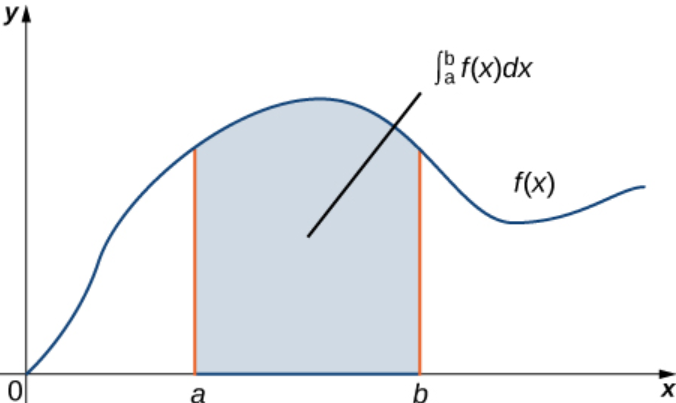
\includegraphics[scale=1]{definite_integrals} 
    \label{definite_int}
\end{figure}

\textbf{Property II : Second Fundamental Theorem of Calculus}

\vspace{5mm}

\begin{tcolorbox}
\begin{center}
\[\int_{a}^{b} f(x).dx = [F(x)]^{b}_{a} = F(b) - F(a) \]
\end{center}
\end{tcolorbox}

\vspace{5mm}

\begin{align}
&\int^{b}_{a} f(x).dx = - \int^{a}_{b} f(x).dx \\[5mm]
&\int^{b}_{a} f(x).dx = \int^{c}_{a} f(x).dx + \int^{b}_{c} f(x).dx \quad \text{where} \: a<c<b \\[5mm]
&\int^{a}_{0}f(x).dx = \int^{a}_{0}f(a-x).dx
\end{align}


\begin{align}
\int^{a}_{-a}f(x).dx = 
\begin{cases}
2.\int^{a}_{0} f(x).dx \quad \text{if} \: f(x) = f(-x) \\
0 \quad if \: f(x) = -f(-x) 
\end{cases}
\end{align}

\vspace{5mm}

\begin{align}
\int^{2a}_{0}f(x).dx = 
\begin{cases}
2.\int^{a}_{0}f(x).dx \quad if \: f(2a-x) = f(x) \\
0 \quad if \: f(2a-x) = -f(x)
\end{cases}
\end{align}

\vspace{5mm}

Mean value of a function in an interval $(a,b)$ is given by:

\begin{tcolorbox}
\begin{center}
$ \displaystyle \frac{1}{b-a} \int_{a}^{b} f(x).dx $
\end{center}
\end{tcolorbox}

\subsection{ Evaluation of Infinite/Improper Integrals}
Consider a definite integral $ \displaystyle \int_{a}^{b} f(x).dx $ - the limits $[a,b]$ are finite and $f(x)$ exists at every point $c \in [a,b]$. The indefinite integral is defined as: \\

\vspace{5mm}

\noindent
\textbf{Type I}
\begin{tcolorbox}
\begin{center}
$ \displaystyle \int_{a}^{\infty} f(x).dx \: \text{or} \: \int_{-\infty}^{b} f(x).dx $
\end{center}
\end{tcolorbox}

\vspace{2mm}
Evaluate $ \displaystyle \lim_{t \to \infty}\int_{a}^{t} f(x).dx $ if it exists and is finite then: \\[3mm]
\begin{tcolorbox}
\begin{center}
$ \displaystyle \int_{a}^{\infty} f(x).dx = \lim_{t \to \infty} \int_{a}^{t} f(x).dx $
\end{center}
\end{tcolorbox}

\vspace{2mm}

Evaluate $ \displaystyle \lim_{t \to -\infty}\int_{t}^{b} f(x).dx $ if it exists and is finite then: \\[3mm]
\begin{tcolorbox}
\begin{center}
$ \displaystyle \int_{-\infty}^{b} f(x).dx = \lim_{t \to -\infty}\int_{t}^{b} f(x).dx $
\end{center}
\end{tcolorbox}

\vspace{5mm}

\noindent
\textbf{Type II} 
\vspace{2mm}
$f(x) \to \infty$ as $x \to a$ at no other point except at $a$. \\[2mm]

\noindent
Evaluate $ \displaystyle \lim_{h \to 0}\int_{a+h}^{b} f(x).dx $ for $f(x) \to \infty$ as $x \to a$ if it exists and is finite then: \\[3mm]

\begin{tcolorbox}
\begin{center}
$ \displaystyle \int_{a}^{b} f(x).dx = \lim_{h \to 0}\int_{a+h}^{b} f(x).dx $ 
\end{center}
\end{tcolorbox}

\noindent
Evaluate $ \displaystyle \lim_{h \to 0}\int_{a}^{b-h} f(x).dx $ for $f(x) \to \infty $ as $x \to b$ if it exists and is finite then: \\[3mm]

\begin{tcolorbox}
\begin{center}
$ \displaystyle \int_{a}^{b} f(x).dx = \lim_{h \to 0}\int_{a}^{b-h} f(x).dx $ 
\end{center}
\end{tcolorbox}

\vspace{5mm}

\noindent
If $ \displaystyle f(x) \to \infty $ at some point $c \in [a,b]$ then: \\[3mm]

\begin{tcolorbox}
\begin{center}
$ \displaystyle \int_{a}^{b} f(x).dx = \int_{a}^{c} f(x).dx + \int_{c}^{b} f(x).dx $
\end{center}
\end{tcolorbox}

\vspace{5mm}

\begin{tcolorbox}
\begin{center}
$ \displaystyle \int_{-\infty}^{\infty} f(x).dx = \int_{-\infty}^{a} f(x).dx + \int_{a}^{\infty} f(x).dx $
\end{center}
\end{tcolorbox}

\vspace{5mm}
\begin{center}
\textbf{***********}
\end{center}

